%%%%%%%%%%%%%%%%%%%%%%%%%%%%%%%%%%%%%%%%%%%%%%%%%%%%%%%%%%%%%%%%%%%%%%%%%%%%%%%%%%%%
% Document data
%%%%%%%%%%%%%%%%%%%%%%%%%%%%%%%%%%%%%%%%%%%%%%%%%%%%%%%%%%%%%%%%%%%%%%%%%%%%%%%%%%%%
\documentclass[12pt]{article} %report allows for chapters
%%%%%%%%%%%%%%%%%%%%%%%%%%%%%%%%%%%%%%%%%%%%%%%%%%%%%%%%%%%%%%%%%%%%%%%%%%%%%%%%%%%%
\usepackage{preamble}

\begin{document}

\begin{center}
   \textsc{\large MATH 271, Homework 10}\\
   \textsc{Due November 22$^\textrm{nd}$}
\end{center}
\vspace{.5cm}

\begin{problem}
Consider the system of linear equations
\begin{align*}
    2x-y-2z&=4\\
    -x + 3y +4z &= -2\\
    2x+y-2z&=8.
\end{align*}
\begin{enumerate}[(a)]
    \item Write this system of equations as a matrix/vector equation
    \[
    [A]\vecv=\boldsymbol{\vec{b}}.
    \]
    \item Solve the system of equations by finding the inverse of the matrix $[A]$.
\end{enumerate}
\end{problem}

\begin{problem}
Consider the matrix
\[
[A] = \begin{pmatrix} 1 & 1 \\ 0 & 2 \end{pmatrix}.
\]
\begin{enumerate}[(a)]
    \item Find the eigenvalues and eigenvectors for this matrix.
    \item Construct the matrix $[P]$ such that
    \[
    [\Lambda] = [P]^{-1}[A][P]
    \]
    from the eigenvectors you found. 
    \item Find $[P]^{-1}$ and compute
    \[
    [P]^{-1}[A][P].
    \]
    Is this $[\Lambda]$ diagonal?
\end{enumerate} 
\end{problem}

\begin{problem}
Consider the matrix
\[
[A]=\begin{pmatrix} 1 & 3 & 0 \\ 3 & 1 & 0 \\
 0 & 4 & 1 \end{pmatrix}
\]
\begin{enumerate}[(a)]
    \item Compute the eigenvalues and eigenvectors for the matrix $[A]$.
    \item Show that $\det([A])=\lambda_1\lambda_2\lambda_3$ and $\tr([A])=\lambda_1 + \lambda_2+\lambda_3$ where $\lambda_1$, $\lambda_2$, and $\lambda_3$ are the eigenvalues you found in (a).
    \item Argue why the eigenvalues of $[A]^{-1}$ must be $\frac{1}{\lambda_1}$, $\frac{1}{\lambda_2}$, and $\frac{1}{\lambda_3}$.
\end{enumerate}
\end{problem}

\begin{problem}
For each description below, construct a single $3\times 3$ transformation matrix.
\begin{enumerate}[(a)]
    \item A rotation by $\frac{\pi}{2}$ in the $yz$-plane.
    \item A rotation by $\frac{\pi}{2}$ in the $xy$-plane, an interchange of the $x$ and $y$ coordinates.
    \item A matrix which undoes everything in part (b).
\end{enumerate}
\end{problem}

\begin{problem}
A matrix in the group of rotation matrices in $\R^2$ (i.e., $\mathrm{SO}(2)$) can be written as
\[
\Rot_\theta = \begin{pmatrix} \cos \theta & - \sin \theta \\ \sin \theta & \cos \theta \end{pmatrix},
\]
for any choice of $\theta$. Another way to think about $\mathrm{SO}(2)$ is to consider it as the rotational symmetry group of the unit circle in the plane.

Next, consider a cyclohexane $C_6H_{12}$ molecule:
    \begin{figure}[H]
        \centering
        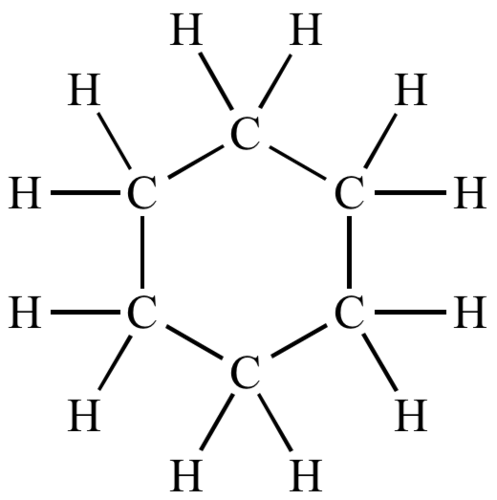
\includegraphics[width=.3\textwidth]{cyclohexane-500x500.png}
    \end{figure}
    \noindent This molecule also has rotational symmetry, but it is a smaller symmetry group than $\mathrm{SO}(2)$. We want to determine this rotational symmetry \emph{subgroup}.
\begin{enumerate}[(a)]
    \item This molecule looks much like a hexagon. Determine the external angles of a hexagon.
    \item Note that if we rotate a hexagon (or cyclohexane) by an external angle, then this leaves the molecule invariant (i.e., it looks no different). Using the internal angle you found, write the rotation matrix for that angle and name this matrix $[g]$.
    \item We can \emph{generate} this group $C_6$ from $[g]$ by repeatedly multiplying $[g]$ with itself.  Show that there are only six elements in this group $C_6$.
    \item These are not all the symmetries of cyclohexane! Explain another symmetry operation that we could use that isn't captured by the rotations above.
\end{enumerate}
If you're interested, look up the group $D_{12}$ which is the \emph{dihedral group of order 12}. Or, taking it further, look at \url{https://en.wikipedia.org/wiki/Cyclohexane_conformation}
\end{problem}

% \begin{problem}
% Consider the second order linear differential equation
% \[
% x''(t)=-x(t).
% \]
% \begin{enumerate}[(a)]
%     \item Let $x'(t)=y(t)$, and write the above differential equation as two first order equations.
%     \item Rewrite the above differential equations as a matrix vector equation
%     \[
%     \begin{pmatrix} x'(t) \\ y'(t) \end{pmatrix} = \begin{pmatrix} a_{11} & a_{12} \\ a_{21} & a_{22} \end{pmatrix} \begin{pmatrix} x(t) \\ y(t) \end{pmatrix},
%     \]
%     by determining the coefficients $a_{ij}$.
%     \item What is the characteristic polynomial for this matrix? 
%     \item Compare the characteristic polynomial of $[A]$ to the characteristic polynomial from the original second order equation given above.
% \end{enumerate}
% \end{problem}

\end{document}